\documentclass{TIJMUjiaoanLL}
\pagestyle{empty}

\begin{document}

\kecheng{分子生物计算}
\neirong{序列和字符串 \ / 第4章}
\jiaoshi{伊现富}
\zhicheng{讲师}
\riqi{2019年9月6\&11日13:30-15:10\&10:00-11:40}
\duixiang{生物医学工程与技术学院2017级生信班(本)}
\renshu{28}
\fangshi{理论讲授}
\xueshi{4}
\jiaocai{Perl语言在生物信息学中的应用——基础篇}

\firstHeader
\maketitle
\thispagestyle{empty}

\mudi{
\begin{itemize}
  \item 掌握:Perl语言的基础知识;标量和数组的使用;字符串的常见操作。
  \item 熟悉:文件的读取;标量上下文和列表上下文。
  \item 了解:Perl语言中双引号和单引号的区别。
  \item 自学:常见函数的高级用法。
\end{itemize}
}

\fenpei{
\begin{itemize}
  \item (5')引言与导入:回顾分子生物学的基础知识,介绍本章将要学习的内容。
  \item (10')序列数据的表征:回顾核酸和蛋白质序列的表征方法,介绍序列和字符串之间的关系。
  \item (30')存储DNA序列:通过存储DNA序列的Perl程序讲解Perl语言的基础知识。
  \item (20')拼接DNA片段:通过拼接DNA片段的Perl程序讲解字符串的拼接操作。
  \item (20')DNA转录成RNA:通过DNA转录成RNA的Perl程序讲解字符串的替换操作。
  \item (5')使用Perl文档:总结查找Perl文档的方法。
  \item (25')序列反向互补:通过获取DNA反向互补序列的Perl程序讲解字符串的翻译反转操作。
  \item (20')从文件读取数据:通过读取文件数据的Perl程序讲解读取文件的基本方法和策略。
  \item (25')数组:通过读取文件中多行数据的Perl程序讲解数组的基本使用与常见操作。
  \item (15')上下文:通过实例介绍上下文的概念,比较标量上下文和列表上下文。
  \item (5')总结与答疑:总结授课内容中的知识点与技能,解答学生疑问。
\end{itemize}
}

\zhongdian{
\begin{itemize}
  \item 重点:Perl语言的基础知识;字符串的常见操作;文件的读取;数组的基本使用。
  \item 难点:字符串的常见操作;数组的基本使用。
  \item 解决策略:通过实例演示帮助学生理解、记忆。
\end{itemize}
}

\waiyu{
\vspace*{-10pt}
\begin{multicols}{2}
字符串(string)

语句(statement)

标量变量(scalar variable)

数组(array)

赋值操作符(assignment operator)

字符串内插(string interpolation)

标量上下文(scalar context)

列表上下文(list context)
\end{multicols}
\vspace*{-10pt}
}

\fuzhu{
\begin{itemize}
  \item 多媒体:序列数据的表征;Perl程序实例;数组的常见操作。
  \item 板书:常见的字符串操作。
  \item 演示:Perl程序实例。
\end{itemize}
}

\sikao{
\vspace*{-10pt}
\begin{multicols}{2}
\begin{itemize}
  \item 列举拼接DNA片段的不同方法。
  \item 比较Perl语言中双引号和单引号的区别。
  \item 列举字符串的常见操作。
  \item 在Perl语言中如何从文件中读取数据?
  \item 列举常见的数组操作。
  \item 举例说明Perl语言中的上下文。
\end{itemize}
\end{multicols}
\vspace*{-10pt}
}

\cankao{
{\footnotesize
\begin{itemize}
  \item Beginning Perl for Bioinformatics, James Tisdall, O'Reilly Media, 2001.
  \item Perl语言入门(第六版),Randal L. Schwartz, brian d foy \& Tom Phoenix著,盛春\ 译,东南大学出版社,2012。
  \item Mastering Perl for Bioinformatics, James Tisdall, O'Reilly Media, 2003.
  \item 维基百科等网络资源。
\end{itemize}
}
}

\firstTail

\newpage
\otherHeader

\begin{enumerate}
  \item 引言与导入(5分钟)
    \begin{enumerate}
      \item 回顾知识点
	\begin{itemize}
	  \item Perl语言:变量,字符串操作符,……
	  \item 分子生物学:中心法则,DNA、RNA和蛋白质
	\end{itemize}
      \item 本章内容
	\begin{itemize}
	  \item Perl语言:标量变量,数组变量,字符串操作,从文件中读取数据
	  \item Perl语言在分子生物学中的应用:拼接DNA片段,DNA转录成RNA,获取DNA的反向互补序列,从文件中读取序列信息,计算序列的统计信息
	\end{itemize}
    \end{enumerate}
  \item 序列数据的表征(10分钟)
    \begin{enumerate}
      \item 序列表征
	\begin{itemize}
\parpic[fr]{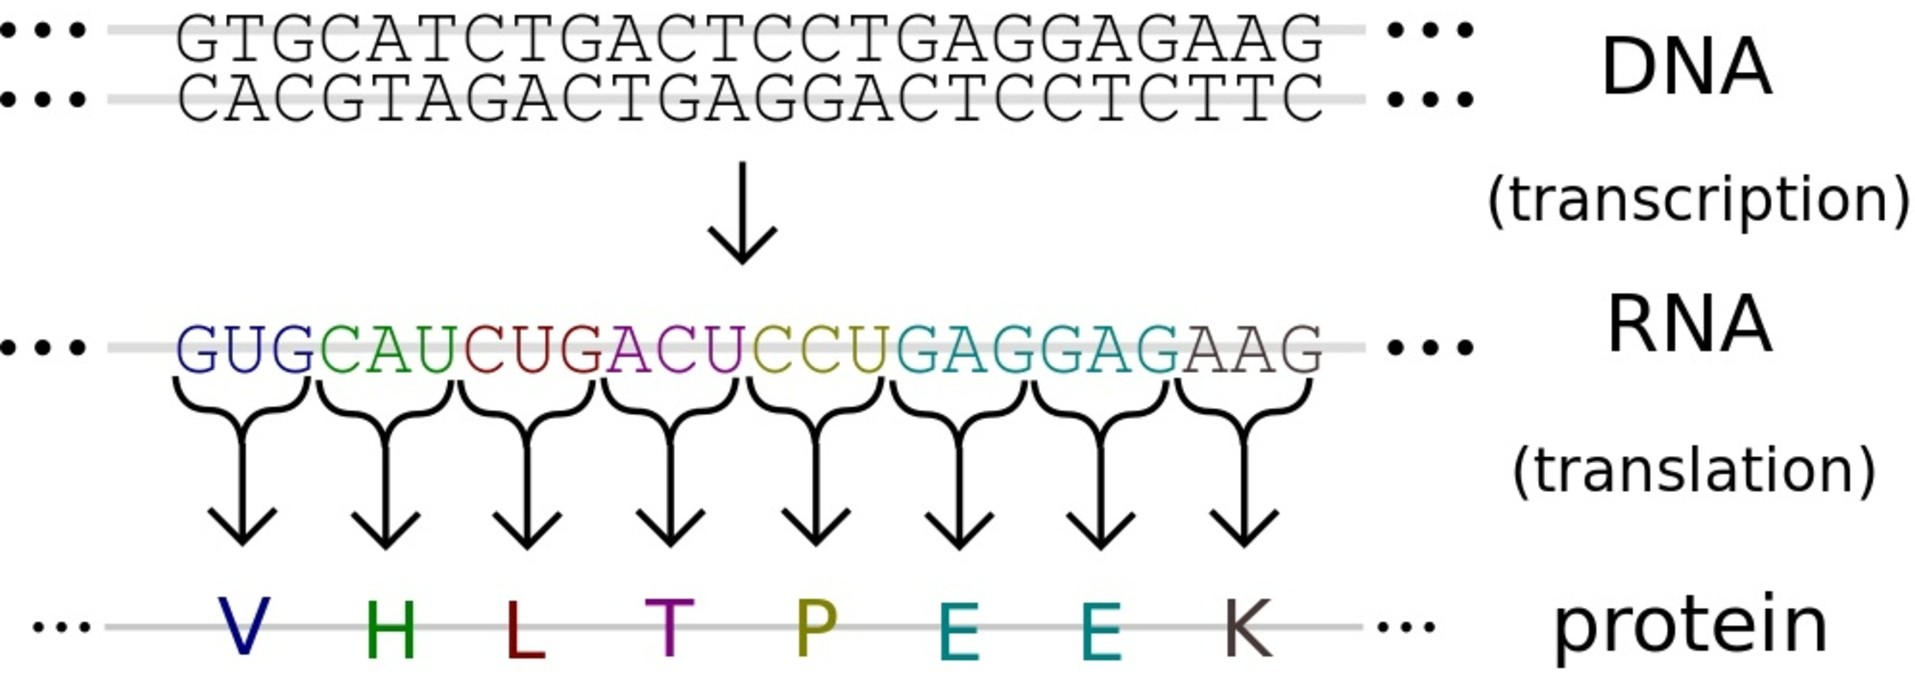
\includegraphics[width=0.45\textwidth]{c4_string_seq_01.jpg}}
	  \item DNA/RNA:A、C、G、T/U、M、R、W、S、Y、K、V、H、D、B、N
	  \item 蛋白质:A、B、C、D、E、F、G、H、I、K、L、M、N、P、Q、R、S、T、V、W、X、Y、Z
	\end{itemize}
      \item 序列与字符串
	\begin{itemize}
	  \item (生物学)DNA/RNA/蛋白质序列 $\Longrightarrow$ (计算机科学)字符串
	\end{itemize}
    \end{enumerate}
  \item 存储DNA序列(30分钟)
    \begin{enumerate}
      \item Perl程序4.1:使用Perl程序存储DNA序列并将其打印出来
      \item \textcolor{red}{【重点】}程序4.1的解释说明\textcolor{red}{(结合程序逐一讲解)}
\vspace*{-1em}
\begin{multicols}{2}
	\begin{itemize}
	  \item 编辑运行:ASCII或纯文本格式;可执行权限
	  \item 控制流:顺序执行;条件/循环流程控制\textcolor{red}{(和RPG中的主线支线相类比)}
	  \item 注释:以 \verb|#|起始,空行和注释会被解释器忽略
	  \item 命令解释:\verb|#!/usr/bin/perl|
	  \item 语句:以 \verb|;|结尾\textcolor{red}{(和中文/英文中的句号相类比)}
	  \item 变量:命名规范;标量变量(以 \verb|$|起始)
	  \item 字符串:单引号 vs. 双引号
	  \item 赋值:\verb|=| vs. \verb|==|
	  \item 打印输出:print,STDOUT
	  \item 退出:\verb|exit;| vs. 自动退出
	\end{itemize}
\end{multicols}
\vspace*{-1em}
    \end{enumerate}
  \item \textcolor{red}{【重点、难点】}拼接DNA片段(20分钟)\textcolor{red}{(结合程序讲解字符串的拼接)}
    \begin{enumerate}
      \item Perl程序4.2:使用Perl程序把两个DNA片段拼接起来\textcolor{red}{(应用:外显子剪接)}
      \item 同样的拼接,不同的方法\textcolor{red}{(方法不止一种,注意开拓思路)}
	\begin{enumerate}
	  \item \verb|$DNA3 = "$DNA1$DNA2"; print "$DNA3\n";|
	  \item \verb|$DNA3 = $DNA1 . $DNA2; print "$DNA3\n";|
	  \item \verb|print $DNA1, $DNA2, "\n";|
	  \item \verb|print "$DNA1$DNA2\n";|
	\end{enumerate}
    \end{enumerate}
  \item \textcolor{red}{【重点、难点】}DNA转录成RNA(20分钟)\textcolor{red}{(结合程序讲解字符串的替换)}
    \begin{enumerate}
      \item 问题转化:(生物学)DNA转录成RNA $\Longrightarrow$ (编程)把DNA序列中的所有T替换成U
      \item Perl程序4.3:使用Perl程序把DNA转录成RNA
      \item 绑定操作符和替换:\verb|$RNA =~ s/T/U/g;|
      \item 方法不止一种
	\begin{enumerate}
	  \item \verb|$RNA = $DNA; $RNA =~ s/T/U/g;|
	  \item \verb|($RNA = $DNA) =~ s/T/U/g;|
	\end{enumerate}
    \end{enumerate}
  \item 使用Perl文档(5分钟)
\vspace*{-1em}
\begin{multicols}{2}
    \begin{enumerate}
      \item 官网:http://www.perl.com
      \item 手册:man perldoc
    \end{enumerate}
\end{multicols}
\vspace*{-1em}

\otherTail
\newpage
\otherHeader

  \item \textcolor{red}{【重点、难点】}序列反向互补(25分钟)\textcolor{red}{(和手工反向互补序列的思路进行比较;结合程序讲解字符串的反转与翻译)}
    \begin{enumerate}
      \item Perl程序4.4:使用Perl程序获取DNA序列的反向互补序列
      \item 两种方法:一错 vs. 一对\textcolor{red}{(出错很正常,关键是找到症结解决问题)};一繁 vs. 一简
      \item 两个函数
	\begin{itemize}
	  \item reverse:反转字符串、数组元素等的顺序
	  \item tr:字符集翻译;\verb|$revcom =~ tr/ACGT/TGCA/;|
	\end{itemize}
    \end{enumerate}
  \item 从文件读取数据(20分钟)
    \begin{enumerate}
      \item 创建数据:文件和文件夹的组织与命名\textcolor{red}{(养成好习惯,终生会收益)}
      \item Perl程序4.5/4.6:使用Perl程序从文件中读取蛋白质序列数据(一行/多行)
      \item \textcolor{red}{【重点】}读取文件\textcolor{red}{(三步走:打开-读取-关闭)}
	\begin{enumerate}
	  \item 关联文件和文件句柄:\verb|open (PROTEINFILE, $proteinfilename);|\textcolor{red}{(文件句柄通常用大写)}
	  \item 通过文件句柄读取文件数据:\verb|$protein = <PROTEINFILE>;|
	  \item 解关联文件和文件句柄:\verb|close PROTEINFILE;|\textcolor{red}{(有开有关、有始有终)}
	\end{enumerate}
    \end{enumerate}
  \item 数组(25分钟)
    \begin{enumerate}
      \item Perl程序4.7:通过数组,使用Perl程序从文件中读取全部的蛋白质序列数据\textcolor{red}{(和4.5/4.6进行比较)}
      \item \textcolor{red}{【重点、难点】}数组操作\textcolor{red}{(演示数组操作实例)}
	\begin{enumerate}
	  \item 标量 vs. 数组:单数 vs. 复数;\verb|$| vs. \verb|@|
	  \item 初始化和输出:\verb|print @bases;| vs. \verb|print "@bases";|
	  \item 元素访问:使用索引,从0开始\textcolor{red}{(编程初期常见错误:从1开始进行索引)}
	  \item 头尾操作:pop,shift,unshift,push
	  \item 其他操作:反转(reverse),获取元素个数(scalar),插入元素(splice)
	\end{enumerate}
    \end{enumerate}
  \item 上下文(15分钟)
    \begin{enumerate}
      \item Perl程序4.8:使用Perl程序演示标量上下文和列表上下文
      \item 上下文\textcolor{red}{(和自然语言中的语境相类比)}
	\begin{itemize}
	  \item 标量上下文:\verb|$a = @bases;| (vs. \verb|$a = scalar @bases;|)
	  \item 列表上下文:\verb|($a) = @bases;|
	\end{itemize}
    \end{enumerate}
  \item 总结与答疑(5分钟)
    \begin{enumerate}
      \item 知识点
	\begin{itemize}
	  \item Perl语言基础:命令解释、注释、语句、赋值、……
	  \item Perl中的变量:标量 vs. 数组
	  \item 字符串操作:拼接,替换,翻译,反转
	  \item 数组:初始化,索引,常见操作
	  \item 上下文:标量上下文 vs. 列表上下文
	\end{itemize}
      \item 技能
	\begin{itemize}
	  \item 编写Perl程序处理DNA序列:存储DNA序列,拼接DNA片段,把DNA转录成RNA,获取DNA的反向互补序列
	  \item 编写Perl程序从文件中读取蛋白质序列数据
	  \item 掌握Perl语言中数组的常见操作
	  \item 灵活运用标量上下文和列表上下文
	\end{itemize}
    \end{enumerate}
\end{enumerate}

\otherTail

%\parpic[fr]{\includegraphics[width=\textwidth]{}}

\end{document}
